\chapter{Applicazione della teoria ecologica alle comunità microbiche}

Gli ecosistemi di comunità microbiche presenti nel corpo umano giocano un ruolo molto importante per la nostra salute\cite{Costello1255}. Ogni individuo può essere visto come un insieme di habitat occupati da comunità microbiche formatesi attraverso i processi fondamentali dell'ecologia: diffusione, diversificazione locale, selezione ambientale e migrazione. I tanti e svariati membri delle comunità hanno un ruolo cruciale nel mantenimento della salute umana liberando essi nutrienti ed energia altrimenti inaccessibili, favorendo la differenziazione dei tessuti, stimolando il sistema immunitario e proteggendo l'ospite dall'invasione da parte di agenti patogeni. 
Un certo numero di disturbi clinici, come l'obesità, la malnutrizione e malattie infiammatorie, sono stati associati all'alterazione della composizione delle comunità microbiche presenti nell'ospite.\\
Il corpo umano, dunque, può essere visto come un ecosistema e la salute di un individuo può essere associata ai servizi forniti
all'organismo dalle comunità microbiche.\\
Recenti scoperte di variazioni inaspettate nella composizione del microbioma di individui sani hanno evidenziato l'importanza di identificare i processi che possano dare origine ad un tale cambiamento: la teoria dell'ecologia cerca di spiegare e predire questi fenomeni. Inoltre, il modello ecologico trasportato nel mondo delle pratiche cliniche può portare ad un miglioramento delle cure fornite ai pazienti: infatti, una visione completa della comunità che si va ad alterare con una certa terapia e non focalizzata solamente sul batterio a cui è dovuto il disturbo, può portare ad un nuovo approccio clinico che nella cura di una malattia tiene conto dell'intero microbioma dell'individuo.

\section{Sequenziamento del DNA degli individui in comunità microbiche}
Ottenere dati di biodiversità per una comunità microbica non è una cosa semplice: dopo averne prelevato una campione, per riconoscere le specie presenti al suo interno è necessario sequenziare il DNA in esso contenuto.\\
Lo sviluppo di tecniche di sequenziamento di nuova generazione (NGS, \emph{next-generation sequencing}) ha portato ad un incremento delle risorse impegnate in questo tipo di ricerca, aumentando rapidamente le nostre conoscenze sulla composizione e sulle funzioni delle popolazioni batteriche in diversi ambienti\cite{shotgun}. Nel contesto clinico, il microbioma dell'intestino umano è stato soggetto ad indagini sofisticate che hanno rivelato una forte interazione tra i microrganismi, il sistema immunitario e il metabolismo. Una ridotta biodiversità o uno squilibrio tra le popolazioni di specie batteriche all'interno comunità microbiche dell'intestino umano sono state associate ad una serie di fenotipi come l'obesità, malattie infiammatorie dell'intestino, diabete di tipo \RNum{2} e numerosi altri disturbi.\\
La maggior parte degli studi riguardanti la comprensione delle dinamiche che governano le popolazioni batteriche sono stati condotti attraverso i cosiddetti approcci metagenomici, che studiano cioè l'insieme dei diversi materiali genetici, in modo semplice ed efficace in termini di costi. I principali metodi di sequenziamento del DNA sono il metodo \emph{shotgun} e il metodo $16S$.
%Ci concentreremo ora sul metodo \emph{shotgun}, in quanto i dati che utilizzeremo successivamente in questo lavoro sono stati ottenuti attraverso questo metodo.
Il metodo \emph{shotgun} è una tecnica sperimentale di sequenziamento dell'intero genoma di un organismo\cite{HEATHER20161}. Poiché a causa dell'elevata lunghezza della sequenza genetica è impossibile sequenziare il genoma in un unico passaggio, esso consiste nella creazione di numerosi piccoli frammenti di DNA che vengono clonati e sequenziati separatamente da entrambi i versi. Questi poi vengono riassemblati \emph{in silico} attraverso criteri di compatibilità e sovrapposizione, in modo da ottenere una lunga sequenza continua. Con il metodo $16S$ invece si va a sequenziare il gene ribosomale $16S$ che da una parte, essendo contenuto in una regione molto conservata, aiuta l'amplificazione, e dall'altra parte,differendo da una specie all'altra, ne permette la classificazione.\\
Le sequenze così ottenute vengono poi confrontate con quelle presenti nei database che contengono le informazioni sui metagenomi dei batteri finora sequenziati. In particolare il progetto microbioma umano (HMP, \emph{human microbiome project}) contiene una vasta raccolta di sequenze di microorganismi associati al corpo umano, inclusi eucarioti, batteri, archei e virus, ottenute sia con il metodo \emph{shotgun} che con il sequenziamento $16S$. Attingendo a queste informazioni è dunque possibile ottenere informazioni su quali specie batteriche siano presenti all'interno di campioni di interesse e con quali abbondanze.



\section{Applicazione dei metodi di \emph{upscaling}}
Dato un campione di $N$ individui (cioè, nel caso di dati metagenomici, di $N$ sequenze di DNA, ovvero i cosiddetti \emph{reads}), grazie ai metodi di classificazione tassonomica sopra citati, è possibile assegnare la specie solamente ad una frazione di questi; le restanti sequenze vengono scartate perché nei database di riferimento non risultano esserci  batteri con tali stringhe di DNA. Analogamente a quanto viene fatto in ecologia, utilizzando i metodi \emph{upscaling} si potrebbe stimare il numero di specie e la loro abbondanza tra questi batteri non identificati, attraverso i dati tassonomici delle specie riconosciute con successo (in una frazione $p^*$). La frazione $p^*$ può essere quindi stimata come il rapporto tra il numero di sequenze che hanno trovato riscontro nel database, $N^*$, e il numero di sequenze inizialmente presenti nel campione, $N$, i.e., $p^*=N^*/N$.  Le specie assenti nel campione di riferimento in ecologia corrispondono quindi, in questo contesto, alle specie a cui appartengono le sequenze che non riescono ad essere classificate.

Per questo lavoro sono stati ottenuti, utilizzando il software Kaiju\cite{Kaiju}, due vettori di abbondanze batteriche a partire da campioni sequenziati con metodo \emph{shotgun}. In particolare un campione riguarda il microbioma un individuo sano mentre l'altro riguarda quello di un individuo affetto dal morbo di Crohn, una malattia dell'intestino. I dati utilizzati sono stati presi dallo studio svolto nell'articolo "Characterization of the gut microbiome using 16S or shotgun metagenomics"\cite{shotgun}. \\

\subsection{Test}
Per sondare l'efficienza nell'ambito delle comunità microbiche dei metodi di \emph{upscaling} precedentemente descritti sono stati condotti dei test su ognuno dei due campioni, procedendo in questo modo:
\begin{itemize}
    \item per ogni campione sono stati selezionati 100 sottocampioni in modo casuale, ognuno contenete l'$1\%$ della popolazione totale;
    
    \item ad ogni sottocampione sono stati applicati i metodi di \emph{upscaling}, i due parametrici della binomiale negativa e della distribuzione logaritmica e il metodo non parametrico $\emph{Chao}_\emph{wor}$, con con $p^*=0.01$;
    
    \item sono stati predetti i numeri di specie alla scala globale (quella del campione) e confrontati con quelli reali che conosciamo a tale scala.
\end{itemize}

Analizzando i risultati dei test abbiamo notato i seguenti fatti:
\begin{itemize}
    \item il metodo $\emph{Chao}_\emph{wor}$ è inapplicabile. Questo infatti si basa sul conteggio del numero di specie rare, popolate cioè da uno o due individui. Nel caso di comunità microbiche non vengono identificate specie con questo tipo di caratteristiche alla sotto-scala analizzata e dunque il metodo non fornisce alcun risultato;
    
    \item il metodo parametrico della distribuzione logaritmica di Fisher sovrastima il numero di specie, in particolare predice circa il doppio del numero di specie realmente presenti nel campione iniziale;
    
    \item il metodo parametrico della binomiale negativa fornisce in tutti i casi analizzati una stima corretta del numero di specie presenti nel campione.
    
\end{itemize}

Sono stati calcolati gli errori percentuali sulle specie predette alla scala globale da ognuno dei 100 sottocampioni. Per il metodo della binomiale negativa questi sono dell'ordine dello $0.01 \%$ e del $2.5 \%$ rispettivamente per l'individuo sano e per l'individuo malato. Il metodo della distribuzione logaritmica produce invece degli errori significativamente grandi: poiché il numero di individui e il numero di specie sono uguali per ogni sottocampione, per ognuna delle $100$ prove questo metodo predice, attraverso le equazioni (\ref{eq:solve}) e (\ref{eq:SalphaLS}), lo stesso numero di specie e dunque gli errori percentuali sono uguali. Questi risultano dell' $ 85 \%$ per l'individuo sano e dell' $ 83 \% $ per l'individuo malato.

\begin{figure}[h]
  \centering
  \begin{minipage}[b]{0.4\textwidth}
    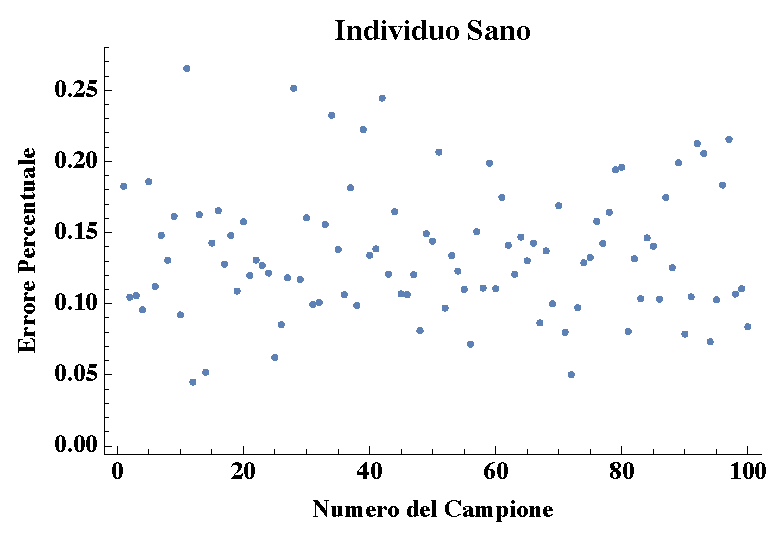
\includegraphics[width=\textwidth]{Figure/erroriHtets.eps}
    \caption{Errore percentuale sulle specie predette da campioni dell'$1 \% $  con il metodo della binomiale negativa per un individuo sano.}
    \label{fig:erroriH}
  \end{minipage}
  \hfill
  \begin{minipage}[b]{0.4\textwidth}
    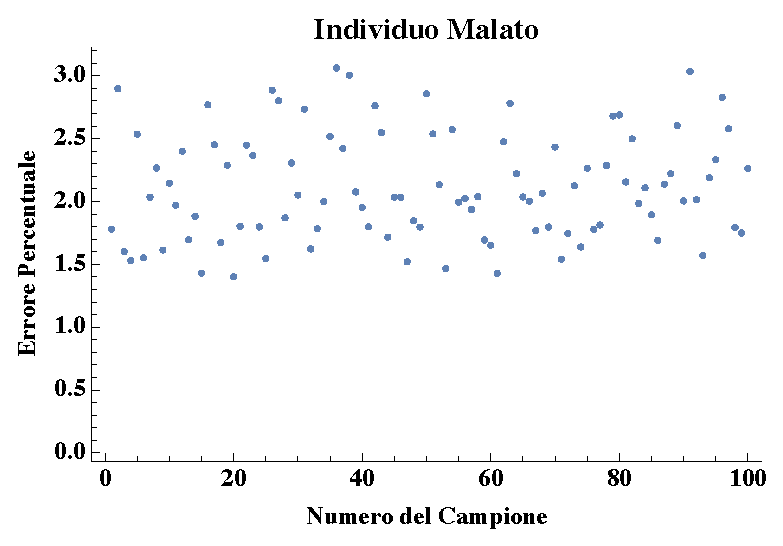
\includegraphics[width=\textwidth]{Figure/erroriCtest.eps}
    \caption{Errore percentuale sulle specie predette da campioni dell'$1 \% $ con il metodo della binomiale negativa per un individuo malato.}
    \label{fig:erroriC}
  \end{minipage}
\end{figure}

Inoltre sono state calcolate le RSA predette a scala globale a partire dai parametri stimati alla scala dei sottocampioni. Si nota che i punti ottenuti per la binomiale negativa riproducono l'andamento della RSA a scala globale, mentre quelli ottenuti per la distribuzione logaritmica non ne predicono il picco.
%\begin{figure}
%\centering
  %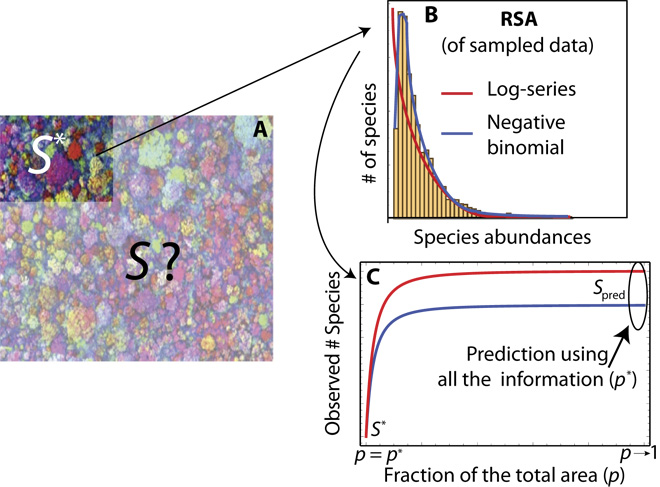
\includegraphics[width=0.6\linewidth]{Figure/RSA.jpg}
  %\caption{\textbf{Rappresentazione schematica del modello di upscaling}. Questo consiste in tre passaggi. (\textbf{A}) Conosciamo l'abbondanza di $S^*$ specie alla scala di campionamento $\emph{p}^*$. (\textbf{B}) Facciamo un fit della SAD con una binomiale negativa o una distribuzione logaritmica. (\textbf{C}) Usando i parametri del miglior fit ottenuti in (B) e usando le equazioni (\ref{eq:SalphaLS}) e (\ref{eq:upscaleNB}) per dedurre la biodiversità dell'intero ecosistema.\cite{Tovoe1701438} }
 % \label{fig:RSA1}
%\end{figure}


\begin{figure}[H]
  \centering
  \begin{minipage}[b]{0.45\textwidth}
    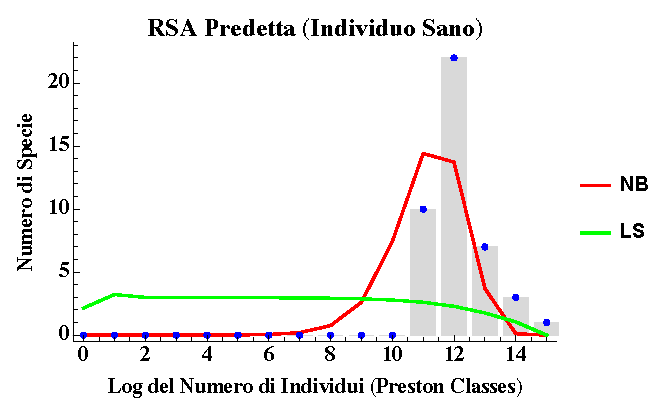
\includegraphics[width=\textwidth]{Figure/rsapredH.eps}
    \caption{RSA predetta per individuo sano. Le previsioni della binomiale negativa riproducono l'andamento reale mentre quelle della distribuzione logaritmica falliscono nel riprodurre il picco.}
    \label{fig:rsapredH}
   \end{minipage}
  \hfill
  \begin{minipage}[b]{0.45\textwidth}
    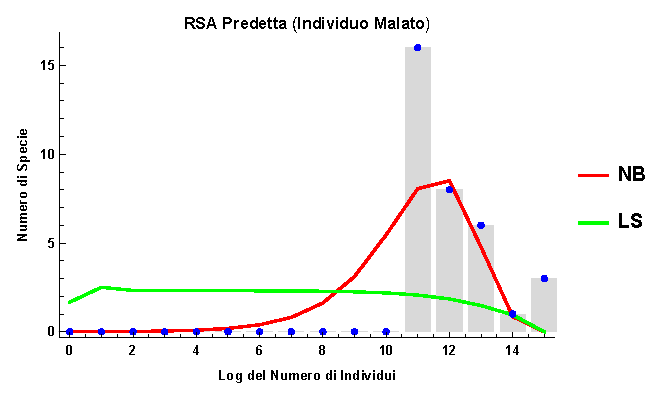
\includegraphics[width=\textwidth]{Figure/rsapredC.eps}
    \caption{RSA predetta per individuo malato. Le previsioni della binomiale negativa riproducono l'andamento reale mentre quelle della distribuzione logaritmica falliscono nel riprodurre il picco.}
    \label{fig:rsapredC}
    \end{minipage}
\end{figure}

Abbiamo sotto-campionato ognuno dei due campioni, selezionando casualmente per $100$ volte il $10 \%, 20 \%,...,90 \%$ degli individui. Per ogni sottocampione è stato poi calcolato il numero di specie predette alla scala globale. In figura \ref{fig:predSpH} e \ref{fig:rsapredC} abbiamo inserito i grafici del numero medio predetto ad ogni sotto-scala per l'individuo sano e malato. Vediamo che il metodo della binomiale negativa predice correttamente il numero di specie anche partendo da campioni a scale ridotte, mentre quello della distribuzione logaritmica si avvicina al valore vero solo per scale molto grandi.

\begin{figure}[H]
  \centering
    \begin{minipage}[b]{0.45\textwidth}
    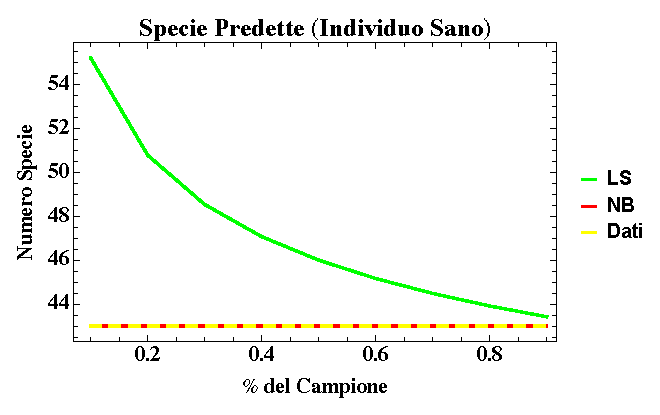
\includegraphics[width=\textwidth]{Figure/cfrpredSpH.eps}
    \caption{Individuo sano. Specie predette a scala globale.}
    \label{fig:predSpH}
    \end{minipage}
\hfill
  \begin{minipage}[b]{0.45\textwidth}
    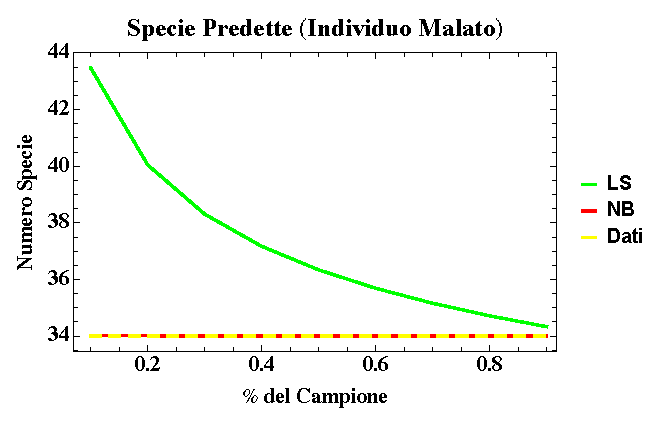
\includegraphics[width=\textwidth]{Figure/cfrpredSpC.eps}
\caption{Individuo malato. Specie predette a scala globale.}
\label{fig:predSpC}
\end{minipage}
\end{figure}

Alla luce dei risultati dei test applichiamo ai nostri campioni solo i due metodi parametrici.\newline

%\begin{table}[]
%\centering
%\begin{tabular}{l|l|l|l|l|}
%\cline{2-5}
%                                     & \textbf{nSpecie} & \textbf{LS} & \textbf{NB} & \textbf{Chao}
%                         \\ \hline
%\multicolumn{1}{|l|}{\textbf{Sano}}  & 43               & 78          & 43          & non applicabile        \\ \hline
%\multicolumn{1}{|l|}{\textbf{Crohn}} & 34.7              & 68          & 34          & non applicabile        \\ \hline
%\end{tabular}
%\caption{Simulazione Sniper Attack}
%\label{Tab:sniperattack}
%\end{table}

\subsection{Risultati di \emph{upscaling}}
Nelle seguenti figure sono rappresentate le RSA dei due campioni. Questi istogrammi, detti \emph{Preston Plot}, rappresentano la distribuzione relativa delle specie raggruppando nell'asse delle ascisse il logaritmo in base due del numero di individui e mostrando nell'asse delle ordinate il numero di specie per ogni classe, cioè per ogni \emph{Preston Class}. Fare un istogramma di Preston significa costruire un sistema di suddivisione in categorie di abbondanze che raddoppiano ($1,2,4,8,16...$) e contare quante specie appartengono alle varie classi. Le specie che hanno esattamente $1,2,8,16..$ individui vanno divise equamente tra le due categorie adiacenti. Questo tipo di classificazione delle specie trasforma effettivamente i dati di abbondanza relativa delle specie nel loro logaritmo in base $2$.


\begin{figure}[H]
  \centering
  \begin{minipage}[b]{0.45\textwidth}
    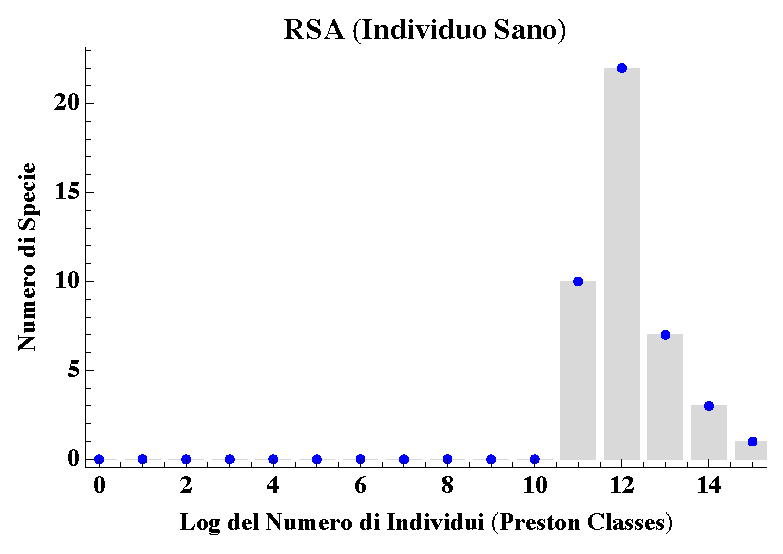
\includegraphics[width=\textwidth]{Figure/RSAH.eps}
    \caption{RSA individuo sano. Preston Plot.}
    \label{fig:RSAH}
  \end{minipage}
  \hfill
  \begin{minipage}[b]{0.45\textwidth}
    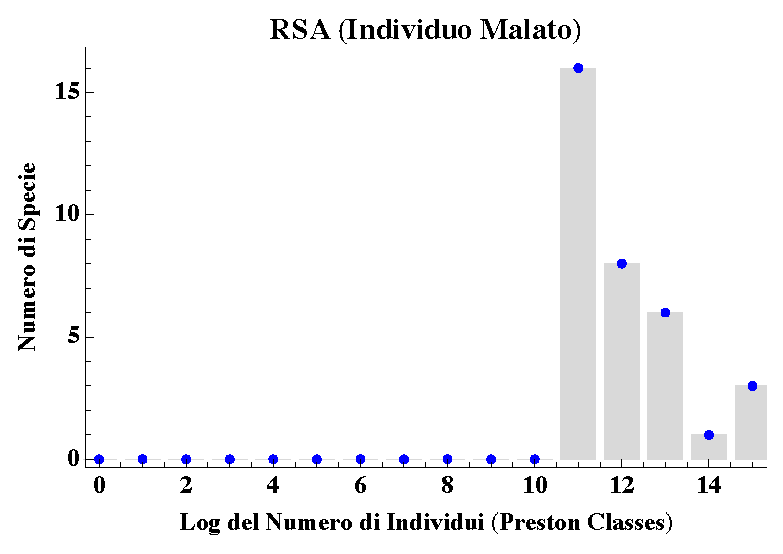
\includegraphics[width=\textwidth]{Figure/RSAC.eps}
    \caption{RSA individuo malato. Preston Plot.}
    \label{fig:RSAC}
  \end{minipage}
\end{figure}

\begin{table}[H]
\centering
\begin{tabular}{l|l|l|l|l|}
\cline{2-5}
                                     & $\mathbf{S^*}$ & $\mathbf{N^*}$ & $\mathbf{N}$ & $\mathbf{p^*}$ \\ \hline
\multicolumn{1}{|l|}{\textbf{Sano}}  & 43                & 176531               & 733551           & 0.240653    \\ \hline
\multicolumn{1}{|l|}{\textbf{Crohn}} & 34                & 159376               & 268205           & 0.594232    \\ \hline
\end{tabular}
\caption{Dati Iniziali.}
\label{Tab:dati}
\end{table}

Nella tabella \ref{Tab:dati} sono indicati, per ognuno dei due campioni, il numero di specie $S^*$ e di individui $N^*$ riconosciuti, il numero di sequenze $N$ ricostruite prima che venissero scartate quelle che non hanno trovato riscontro nel database e la $p^*$ corrispondente, stimata come $p^*=N^*/N$.


Assumendo per la RSA una forma binomiale negativa e fittando il corrispondente pattern empirico otteniamo i seguenti parametri:


\begin{table}[H]
\centering
\begin{tabular}{l|l|l|l|}
\cline{2-4}
                                     & \textit{r}    & $\mathbf{\hat \xi}_{p^*}$                & $\mathbf{\xi}$             \\ \hline
\multicolumn{1}{|l|}{\textbf{Sano}}  & $2.4 \pm 0.4$ & $0.9994 \pm 0.0001$ & $0.99986 \pm0.00003 $ \\ \hline
\multicolumn{1}{|l|}{\textbf{Crohn}} & $1.2 \pm 0.3$ & $0.99975 \pm0.00007 $     & $0.99985 \pm0.00004 $ \\ \hline
\end{tabular}
\caption{Parametri Binomiale Negativa.}
\label{Tab:parametriNB}
\end{table}

Assumendo invece una distribuzione logaritmica otteniamo:

\begin{table}[H]
\centering
\begin{tabular}{l|l|l|}
\cline{2-3}
                                     & $\hat x_{p^*}$                    & $x$ \\ \hline
\multicolumn{1}{|l|}{\textbf{Sano}}  & $0.999 \pm 0.002$     & $ 0.999995 \pm 0.000004$ \\ \hline
\multicolumn{1}{|l|}{\textbf{Crohn}} & $0.99998 \pm 0.00002$ & $ 0.99999 \pm0.00001$  \\ \hline
\end{tabular}
\caption{Parametri Distribuzione Logaritmica.}
\label{Tab:parametriLS}
\end{table}

dove $\xi$ e $x$ sono i parametri delle distribuzione a scala globale calcolati con le equazioni (\ref{eq:NBparameter}) e (\ref{eq:LSparameter}) rispettivamente.

In figura \ref{fig:plotRSAH} e \ref{fig:plotRSAC} possiamo vedere le RSA ottenute fittando i parametri alla scala del campione (tabelle \ref{Tab:parametriNB} e \ref{Tab:parametriLS}).

\begin{figure}[H]
  \centering
  \begin{minipage}[b]{0.45\textwidth}
    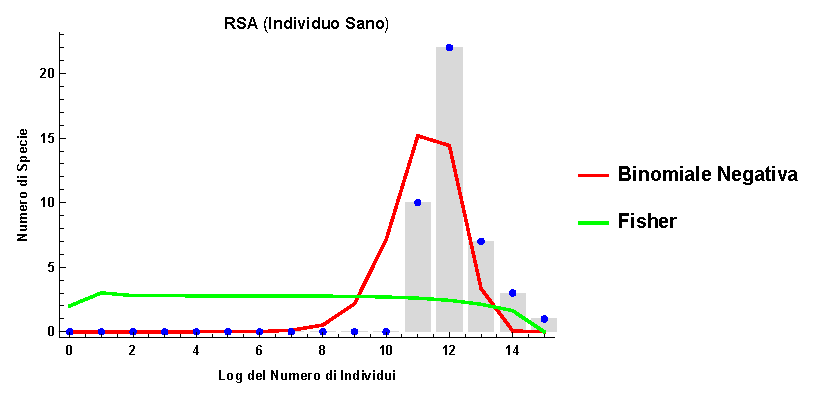
\includegraphics[width=\textwidth]{Figure/rsaplotH.eps}
    \caption{RSA individuo sano: Preston Plot e curve di fit.}
    \label{fig:plotRSAH}
  \end{minipage}
  \hfill
  \begin{minipage}[b]{0.45\textwidth}
    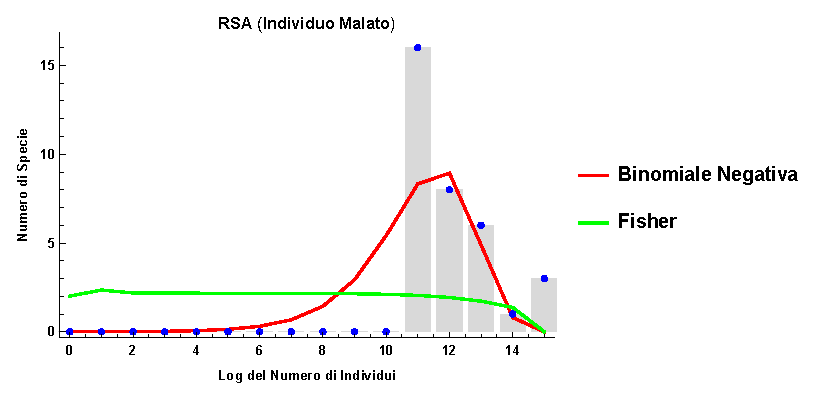
\includegraphics[width=\textwidth]{Figure/rsaplotC.eps}
    \caption{RSA individuo malato: Preston Plot e curve di fit.}
    \label{fig:plotRSAC}
  \end{minipage}
\end{figure}

Per calcolare il numero di specie con una data abbondanza $k$ abbiamo calcolato le (\ref{eq:NBprobability}) e (\ref{eq:fisherdist}) di parametri ottenuti dai fit per $n=k$ e moltiplicato il risultato per il numero di specie presenti nel campione di riferimento.


Anche in questo caso, a differenza della distribuzione logaritmica, la binomiale negativa riproduce la reale distribuzione delle specie.

Abbiamo poi calcolato il numero di specie predetto alla scala globale, $p=1$, ottenendo i risultati mostrati nella seguente tabella:

\begin{table}[H]
\centering
\begin{tabular}{l|l|l|l|}
\cline{2-4}
                                     & $S^*$ & $S_{NB}$ & $S_{LS}$ \\ \hline
\multicolumn{1}{|l|}{\textbf{Sano}}  & 43  & 43       & 48       \\ \hline
\multicolumn{1}{|l|}{\textbf{Crohn}} & 34  & 34       & 35       \\ \hline
\end{tabular}
\caption{Risultati di upscaling.}
\label{Tab:risultatiup}
\end{table}

Notiamo che, sia per l'individuo sano sia per quello affetto da morbo di Crohn, con il metodo della binomiale negativa il numero di specie predette alla scala globale coincide con il numero di specie realmente presenti nel campione, mentre il numero predetto dal metodo della distribuzione di Fisher si discosta poco dal valore di $S^*$.\\
Questi risultati sono ragionevoli se si guarda la SAR dei campioni. Per entrambi i campioni abbiamo selezionato casualmente, per ognuna delle scale del $10\%,20\%,...,90\%$, 100 sottocampioni. In media, ad ogni scala, si trova che il numero di specie presenti nei sottocampioni coincide con quello delle specie presenti alla scala del campione di riferimento. I risultati di \emph{upscaling} sono dunque compatibili con questa evidenza. 